\begin{frame}[allowframebreaks,allowdisplaybreaks]
    \subsection{Secondary Memory Access}
    \frametitle{B-Tree Secondary Memory Access}
    \begin{columns}
        \begin{column}{.7\textwidth}
            \begin{block}{}
                \begin{itemize}
                    \item The B-Tree is fairly good for storing data in external memory in comparison to height, weight or search trees.
                    \item The limit of \(2\alpha\) keys help us by having a balance availability and fragmentation of the data.
                    \item But, this limit also make that if we need to re-balance the tree the 
                        operation will take \(\Theta\left(\alpha \log n\right)\), updating all the split nodes.
                    \item This operation doesn't affect much in main memory, 
                        but in secondary memory where the access time isn't always constant 
                    \item Each read on the secondary memory can make a lot of problems in the execution of the code.
                \end{itemize}
            \end{block}
        \end{column}
        \begin{column}{.35\textwidth}
            \begin{block}{}
                \begin{figure}[h!]
                    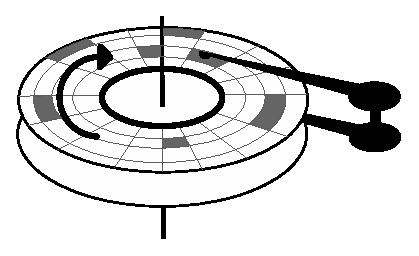
\includegraphics[width=\linewidth]{resources/made/external_storage_wblocks.eps}
                    \caption{External storage with the sectors to access highlighted}
                \end{figure}
            \end{block}
        \end{column}
    \end{columns}

    \framebreak{}
    \begin{center}
    \begin{tabular}{c@{|}ccccccc}
        \toprule
                       & Retrival & Insertion w/ overflow & Deletion w/ underfull \\
            \midrule
            \(\Omega\) & \(t = 1\) \(w = 0\) & \(t = h\) \(w = 1\) & \(t = h\) \(w = 1\) \\
            \midrule
            \(\Theta\) & \(t \leq h\) \(w = 0\) & \(t \leq h + 2 + \frac{2}{\alpha}\) \(w \leq 3 + \frac{2}{\alpha}\) & \(t \leq 3h - 2\) \(w \leq 2h +1\) \\
            \midrule
            \(O\) & \(t = h\) \(w = 0\) & \(t = 3h - 2\) \(w = 2h + 1\) & \(t = 3h - 2\) \(w = 2h + 1\) \\
        \toprule
    \end{tabular}
    \begin{itemize}
        \item Where \(t\) is the number of fetch and readings of nodes on the secondary memory.
        \item And \(w\) is the number of writings of nodes on the secondary memory.
    \end{itemize}
        \cite{bayer_organization_1972}
    \end{center}
\end{frame}
